\documentclass{carve}
\begin{document}

\title{Carve Documentation}
\author{Tobias Sargeant}

\frontmatter

\maketitle

\cleardoublepage\tableofcontents
\cleardoublepage\listoffigures
\cleardoublepage\listoftables
\cleardoublepage\lstlistoflistings

\mainmatter

\chapter{Representation of polyhedra}

Carve polyhedra are defined by collections of vertices (instances of
\code{carve::poly::Vertex}) that define points in 3-dimensional space,
and collections of faces (instances of \code{carve::poly::Face}) that
define the connectivity of vertices. Because faces refer to vertices
by pointer, vertex identity is determined by address rather than by
location in 3-dimensional space.

Faces are oriented anticlockwise in a right handed coordinate
system. Although a face may consist of more than three vertices, all
vertices of any given face must lie on a single plane.

A polyhedron defined by a set of faces and vertices consists of one or
more connected surfaces. The decomposition of a set of faces into
surfaces is computed automatically, and shared vertices
(\fref{fig:polyhedron-shared-vertex}) and edges
(\fref{fig:polyhedron-shared-edge}) are handled correctly. A
polyhedron may not, however, be self intersecting.

Each surface is either ``closed'' or ``open''. A closed surface obeys
the property that for every edge (determined by a pair of consecutive
vertices forming part of a face) there exists an edge of the opposite
orientation that is part of some other face.

A closed surface bounds a non-zero (possibly infinite) volume of
space. The space defined by a surface depends upon the orientation of
its defining faces. By inverting the vertex order of all faces of a
closed surface, the complementary volume is created. For example, a
cube with faces ordered clockwise in a right-handed coordinate system
describes the infinite volume consisting of all space except that
delimited by the cube.

Used carefully, more than one closed surface may be combined to create
a shell. A surface representing an infinite volume enclosed within a
surface representing a finite volume represents a hollow solid, and
such solids are handled correctly during CSG operations.

\begin{figure}
  \begin{center}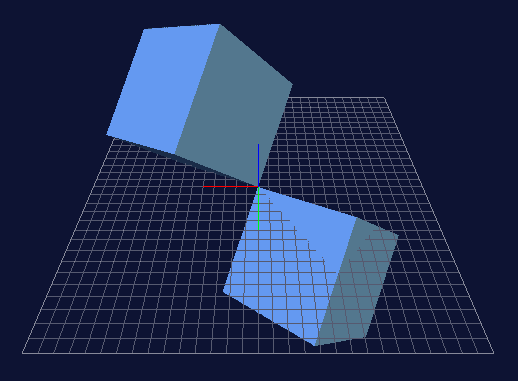
\includegraphics[width=3.453in]{polyhedra/shared-vertex.png}\end{center}
  \caption{A polyhedron consisting of two surfaces sharing a vertex}
  \label{fig:polyhedron-shared-vertex}
\end{figure}

\begin{figure}
  \begin{center}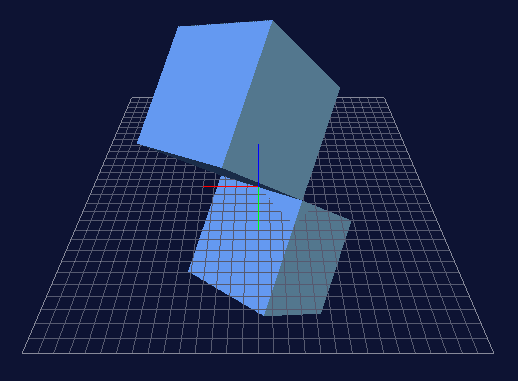
\includegraphics[width=3.453in]{polyhedra/shared-edge.png}\end{center}
  \caption{A polyhedron consisting of two surfaces sharing an edge}
  \label{fig:polyhedron-shared-edge}
\end{figure}

\begin{section}{Construction of Polyhedra}

A polyhedron may be constructed in a number of ways.

In the first case (Listing \ref{code:poly-ctor-1}) a vector of faces
and a vector of vertices is provided. The vertices pointed to by the
faces in \code{\_faces} must be members of the vector of vertices,
\code{\_vertices}. Ownership is taken of the face and vertex vectors,
so as to avoid unnecessary copies. On return, both vectors will be
empty.

\begin{lstlisting}[language=C++,float,caption=\code{carve::poly::Polyhedron} constructor 1,label=code:poly-ctor-1]
carve::poly::Polyhedron(
    std::vector<carve::poly::Face *> &_faces,
    std::vector<carve::poly::Vertex> &_vertices,
    bool _recalc = false);
\end{lstlisting}

\begin{lstlisting}[language=C++,float,caption=\code{carve::poly::Polyhedron} constructor 2,label=code:poly-ctor-2]
carve::poly::Polyhedron(
    std::vector<carve::poly::Face *> &_faces,
    bool _recalc = false);
\end{lstlisting}

\begin{lstlisting}[language=C++,float,caption=\code{carve::poly::Polyhedron} constructor 3,label=code:poly-ctor-3]
carve::poly::Polyhedron(
    std::list<carve::poly::Face *> &_faces,
    bool _recalc = false);
\end{lstlisting}

\begin{lstlisting}[language=C++,float,caption=\code{carve::poly::Polyhedron} constructor 4,label=code:poly-ctor-4]
carve::poly::Polyhedron(
    const std::vector<carve::geom3d::Vector> &vertices,
    int n_faces,
    const std::vector<int> &face_indices);
\end{lstlisting}

\begin{lstlisting}[float,language=C++,caption=Constructing a cube directly,label=code:cube-direct]
#include <carve/polyhedron.hpp>

carve::poly::Polyhedron *makeCube(
    const carve::math::Matrix &t = carve::math::Matrix()) {

  std::vector<carve::poly::Vertex> verts;
  std::vector<carve::poly::Face *> faces;
  
  verts.reserve(8);
  faces.reserve(6);

  verts.push_back(
    carve::poly::Vertex(t * carve::geom::VECTOR(+1.0, +1.0, +1.0)));
  verts.push_back(
    carve::poly::Vertex(t * carve::geom::VECTOR(-1.0, +1.0, +1.0)));
  verts.push_back(
    carve::poly::Vertex(t * carve::geom::VECTOR(-1.0, -1.0, +1.0)));
  verts.push_back(
    carve::poly::Vertex(t * carve::geom::VECTOR(+1.0, -1.0, +1.0)));
  verts.push_back(
    carve::poly::Vertex(t * carve::geom::VECTOR(+1.0, +1.0, -1.0)));
  verts.push_back(
    carve::poly::Vertex(t * carve::geom::VECTOR(-1.0, +1.0, -1.0)));
  verts.push_back(
    carve::poly::Vertex(t * carve::geom::VECTOR(-1.0, -1.0, -1.0)));
  verts.push_back(
    carve::poly::Vertex(t * carve::geom::VECTOR(+1.0, -1.0, -1.0)));

  faces.push_back(
    new Face(&verts[0], &verts[1], &verts[2], &verts[3]));
  faces.push_back(
    new Face(&verts[7], &verts[6], &verts[5], &verts[4]));
  faces.push_back(
    new Face(&verts[0], &verts[4], &verts[5], &verts[1]));
  faces.push_back(
    new Face(&verts[1], &verts[5], &verts[6], &verts[2]));
  faces.push_back(
    new Face(&verts[2], &verts[6], &verts[7], &verts[3]));
  faces.push_back(
    new Face(&verts[3], &verts[7], &verts[4], &verts[0]));

  // note that carve::poly::Polyhedron takes ownership of face
  // pointers and the contents of the vertex array.
  return new carve::poly::Polyhedron(faces, vertices);
}
\end{lstlisting}

\begin{lstlisting}[float,language=C++,caption=Constructing a cube using {\codefont carve::input::PolyhedronData}]
#include <carve/input.hpp>
#include <carve/polyhedron.hpp>

carve::poly::Polyhedron *makeCube(
    const carve::math::Matrix &t = carve::math::Matrix()) {

  carve::input::PolyhedronData data;
  
  data.addVertex(t * carve::geom::VECTOR(+1.0, +1.0, +1.0));
  data.addVertex(t * carve::geom::VECTOR(-1.0, +1.0, +1.0));
  data.addVertex(t * carve::geom::VECTOR(-1.0, -1.0, +1.0));
  data.addVertex(t * carve::geom::VECTOR(+1.0, -1.0, +1.0));
  data.addVertex(t * carve::geom::VECTOR(+1.0, +1.0, -1.0));
  data.addVertex(t * carve::geom::VECTOR(-1.0, +1.0, -1.0));
  data.addVertex(t * carve::geom::VECTOR(-1.0, -1.0, -1.0));
  data.addVertex(t * carve::geom::VECTOR(+1.0, -1.0, -1.0));

  data.addFace(0, 1, 2, 3);
  data.addFace(7, 6, 5, 4);
  data.addFace(0, 4, 5, 1);
  data.addFace(1, 5, 6, 2);
  data.addFace(2, 6, 7, 3);
  data.addFace(3, 7, 4, 0);

  return data.create();
}
\end{lstlisting}

\end{section}

\chapter{CSG Operations}

The \code{carve::csg::CSG} class is responsible for managing CSG
calculations. It provides methods for CSG binary computations between
both closed and open polyhedra, as well as divison of polyhedra by
their common line of intersection. The operation computed by methods
of the \code{carve::csg::CSG} class may be chosen from the standard
primitive binary operations or may be defined by the caller.

The CSG computation may be influenced by the registration of hook
objects that can be used to perform such tasks as triangulation of
result faces and transfer and interpolation of attributes from source
polyhedra to the result.

\begin{section}{CSG Operations on Closed Manifolds}

The \code{compute} method of \code{carve::csg::CSG} has two prototypes:

\begin{lstlisting}[language=C++]
carve::poly::Polyhedron  *compute(
    const carve::poly::Polyhedron  *a,
    const carve::poly::Polyhedron  *b,
    carve::csg::CSG::OP op,
    carve::csg::V2Set *shared_edges = NULL,
    carve::csg::CSG::CLASSIFY_TYPE classify_type = CLASSIFY_NORMAL);
\end{lstlisting}

\begin{lstlisting}[language=C++]
carve::poly::Polyhedron  *compute(
    const carve::poly::Polyhedron  *a,
    const carve::poly::Polyhedron  *b,
    carve::csg::CSG::Collector &collector,
    carve::csg::V2Set *shared_edges = NULL,
    carve::csg::CSG::CLASSIFY_TYPE classify_type = CLASSIFY_NORMAL);
\end{lstlisting}

These methods compute a boolean operation between polyhedra \code{a}
and \code{b}. In the first case, the operation is determined by the
enumeration \code{carve::csg::CSG::OP}, which can take the values:

\begin{itemize}
\item \code{UNION}
\item \code{INTERSECTION}
\item \code{A\_MINUS\_B}
\item \code{B\_MINUS\_A}
\item \code{SYMMETRIC\_DIFFERENCE}
\end{itemize}

\noindent Results for these boolean operations are shown in
\tref{tab:input-polyhedra} and \tref{tab:csg-results}.

\begin{table}
  \begin{center}
    \begin{tabular}{m{2.2in}m{3in}}
      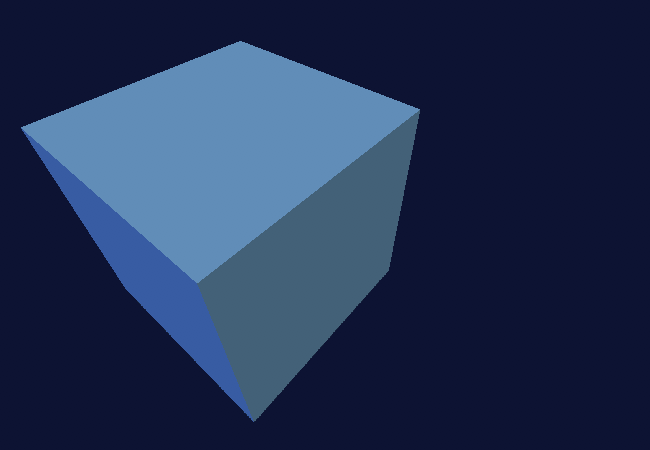
\includegraphics[width=2.167in]{ops/a.png} & \vfill Manifold A \vfill \\
      
\includegraphics[width=2.167in]{ops/b.png} & Manifold B \\
    \end{tabular}
  \end{center}
  \caption{Input polyhedra.}
  \label{tab:input-polyhedra}
\end{table}

\begin{table}
  \begin{center}
    \begin{tabular}{m{2.2in}m{3in}}
      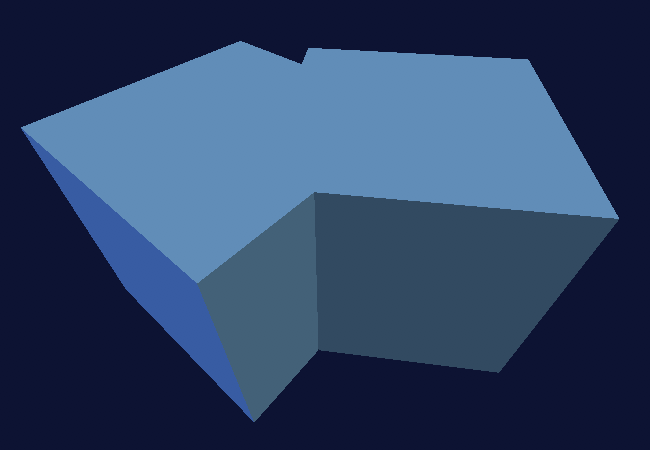
\includegraphics[width=2.167in]{ops/a_union_b.png} &
      Operation: Union (A | B) \newline Enumeration: \code{carve::CSG::UNION} \\
      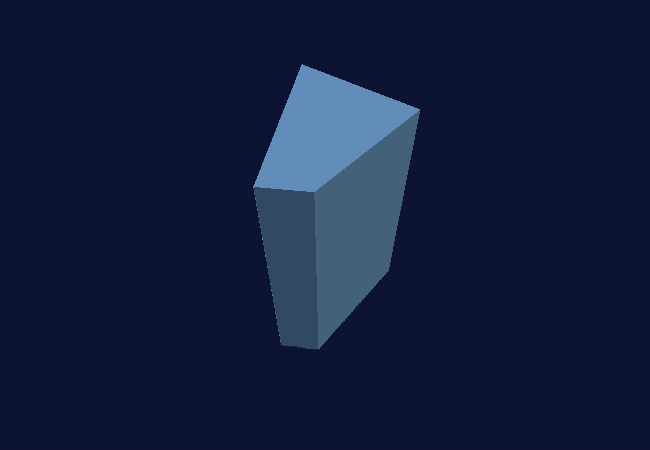
\includegraphics[width=2.167in]{ops/a_intersection_b.png} &
      Operation: Intersection (A \& B) \newline Enumeration: \code{carve::CSG::INTERSECTION} \\
      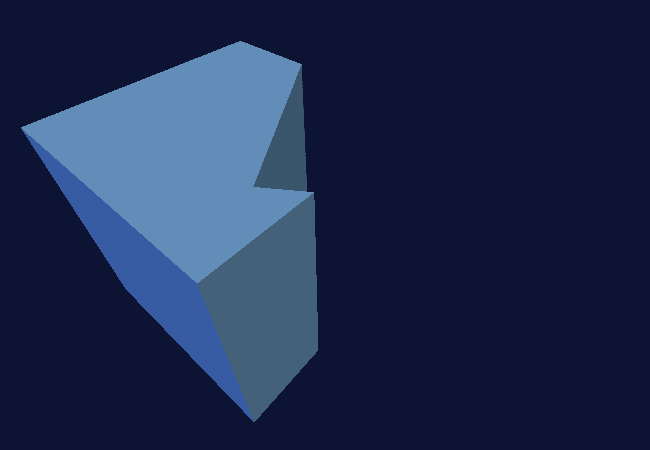
\includegraphics[width=2.167in]{ops/a_minus_b.png} &
      Operation: Difference (A - B) \newline Enumeration: \code{carve::CSG::A\_MINUS\_B} \\
      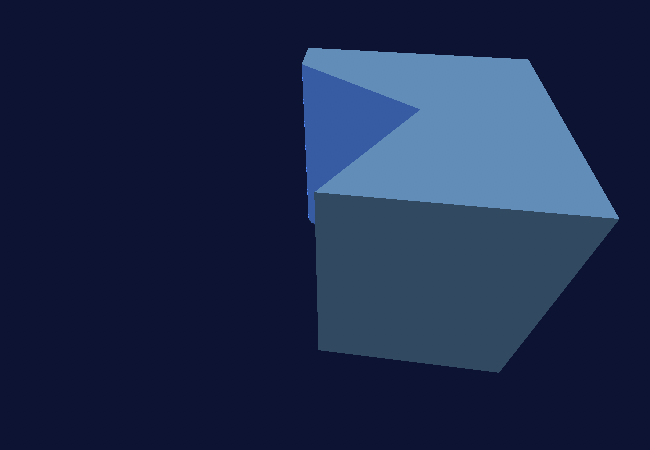
\includegraphics[width=2.167in]{ops/b_minus_a.png} &
      Operation: Difference (B - A) \newline Enumeration: \code{carve::CSG::B\_MINUS\_A} \\
      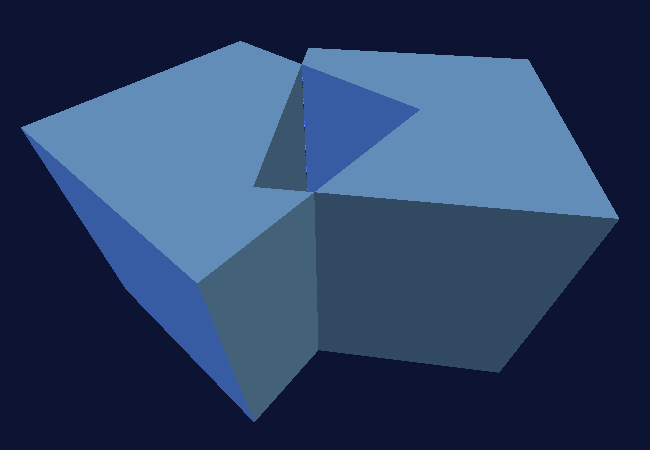
\includegraphics[width=2.167in]{ops/a_xor_b.png} &
      Operation: Symmetric Difference (A B) \newline Enumeration: \code{carve::CSG::SYMMETRIC\_DIFFERENCE} \\
    \end{tabular}
  \end{center}
  \caption{The result of predefined CSG operations.}
  \label{tab:csg-results}
\end{table}

In the second case, the result is determined by a custom
collector. Custom collectors allow the caller to programatically
define which regions of the intersected input polyhedra appear in the
output.

The \code{shared\_edges} parameter provides a way to access the
computed set of edges that defines the point of intersection of the
two polyhedra.

The algorithm used to classify connected components of the intersected
polyhedra is determined by the parameter \code{classify\_type}. The
type of \code{classify\_type} is an enumeration taking values from the
set \{\code{CLASSIFY\_NORMAL}, \code{CLASSIFY\_EDGE}\}.

The classifier is responsible for classifying portions of each
polyhedron bounded by the line of intersection as either:

\begin{itemize}
\item \code{carve::csg::FACE\_OUT} \newline
  The group is outside the space defined by the opposing polyhedron.
\item \code{carve::csg::FACE\_IN} \newline
  The group is inside the space defined by the opposing polyhedron.
\item \code{carve::csg::FACE\_ON\_ORIENT\_IN} \newline
  The group is lying on the surface of the opposing polyhedron, oriented towards its interior.
\item \code{carve::csg::FACE\_ON\_ORIENT\_OUT} \newline
  The group is lying on the surface of the opposing polyhedron, oriented towards its exterior.
\end{itemize}

\noindent with respect to (each surface of) the opposing polyhedron.

\end{section}

\begin{section}{CSG Operations on Open Manifolds}

\end{section}

\chapter{Attribute Interpolation}

\begin{lstlisting}[float,language=C++,caption=Associating texture coordinates with a cube]
#include <carve/interpolator.hpp>

struct tex_t {
  float u, v;

  tex_t() : u(0.0f), v(0.0f) { }
  tex_t(float _u, float _v) : u(_u), v(_v) { }
};

// interpolated attributes must support scalar multiplication.
tex_t operator*(double s, const tex_t &t) {
    return tex_t(t.u * s, t.v * s);
}

// interpolated attributes must support operator+=.
tex_t &operator+=(tex_t &t1, const tex_t &t2) {
    t1.u += t2.u; t1.v += t2.v;
    return t1;
}

void associateTextureVertices(
    carve::poly::Polyhedron *cube,
    carve::interpolate::FaceVertexAttr<tex_t> &fv_tex) {

  fv_tex.setAttribute(cube->faces[0], 0, tex_t(1.0f, 1.0f));
  fv_tex.setAttribute(cube->faces[0], 1, tex_t(0.0f, 1.0f));
  fv_tex.setAttribute(cube->faces[0], 2, tex_t(0.0f, 0.0f));
  fv_tex.setAttribute(cube->faces[0], 3, tex_t(1.0f, 0.0f));

  // ... continue to record other texture coordinates by
  //     face pointer and vertex number.
}
\end{lstlisting}

\begin{lstlisting}[float,language=C++,caption=Interpolating texture coordinates during a CSG operation]
#include <carve/csg.hpp>

carve::poly::Polyhedron *doCSG() {
  carve::poly::Polyhedron *result;

  carve::poly::Polyhedron *cube_1 = makeCube();
  carve::poly::Polyhedron *cube_2 = makeCube(
    carve::math::Matrix::ROT(.4, .2, .3, .4));

  carve::interpolate::FaceVertexAttr<tex_t> fv_tex;
  associateTextureVertices(cube_1, fv_tex);

  carve::csg::CSG csg;
  fv_tex.installHooks(csg);
  result = csg.compute(cube_1, cube_2, carve::csg::CSG::A_MINUS_B);
}
\end{lstlisting}

\appendix

\backmatter

\end{document}
